%++++++++++++++++++++++++++++++++++++++++
% Don't modify this section unless you know what you're doing!
\documentclass[letterpaper,12pt]{article}
\usepackage{tabularx} % extra features for tabular environment
\usepackage{amsmath}  % improve math presentation
\usepackage{graphicx} % takes care of graphic including machinery
\usepackage[margin=1in,letterpaper]{geometry} % decreases margins
\usepackage{cite} % takes care of citations
\usepackage[final]{hyperref} % adds hyper links inside the generated pdf file
\usepackage[numbib,nottoc]{tocbibind}
\usepackage{float}
\usepackage{longtable}
\usepackage{listings}
\usepackage{makeidx}
\usepackage[utf8]{inputenc}
\usepackage{csvsimple}
\hypersetup{
	colorlinks=true,       % false: boxed links; true: colored links
	linkcolor=blue,        % color of internal links
	citecolor=blue,        % color of links to bibliography
	filecolor=magenta,     % color of file links
	urlcolor=blue         
}
%++++++++++++++++++++++++++++++++++++++++

\makeindex

\begin{document}

\title{ADMT 2018 - Project report}
\author{Group 02: Andreas Vieider (13177) \& Laurin Stricker (13412)}
\date{\today}
\maketitle

\tableofcontents
\listoffigures
\listoftables
\cleardoublepage

% \begin{abstract}

% \end{abstract}

\section{Introduction}

The domain of our fictional company is the one of furniture production and retail. The company is located in the province of Bolzano and has several showrooms in the area and one production center.

\subsection{Business processes}

\subsubsection{CRM - Showroom visit}

One CRM process is the collection of data about visitors at the different showrooms. A visitor can either be one who is just looking around without intention of buying anything (Seeleute), a future potential customer or an already existing customer. A visit can lead to an order.

Business questions:
\begin{itemize}
        \item Which is the best running showroom (most visitors, most orders, etc.)
        \item Where are the customers from (with different granularity)
        \item Which department are the customers the most interested in
        \item Compare the number of visitors to the number of customers for a time period and/or showroom
\end{itemize}

\subsubsection{Production}

The company logs every step in the production process, especially duration, defects and machine failures.

Business questions:
\begin{itemize}
        \item What is the average time to produce a particular product
        \item Which is the product with the highest/lowest quality
        \item How much does a product cost in terms of raw material cost
\end{itemize}

\section{Conceptual Design}

The first fact of our Data Warehouse represents a showroom visit. The company is registering each visit in a particular showroom and is interested in some very specific details about a the visit. Namely, for each visit they store the date, the visitor and visitor type, the showroom, the department in which the visitor was particularly interested, the order if the visitor placed one, the sales representative who took care about the visitor and the duration and the number of people with respect to the visit.

The second fact collects some relevant information of a production stage. For each production stage of a particular product, in addition to those two information, also start- and end-date, the machine, the result of the quality control, the operator, the costs of the raw material and the duration of the process are stored.

\begingroup
\renewcommand\arraystretch{0.5}
\begin{longtable}{p{3cm}p{6cm}p{4cm}}
        \caption{Fact table} \\
        Fact & Dimensions & Measures \\
        \endfirsthead \\
        Fact & Dimensions & Measures \\
        \endhead \\
        \hline \\
        Showroom visit & Date, Showroom, Visitor, Visitor type, Order, Department, Sales representative & Duration (AVG - additive), Amount of people (SUM - additive, AVG - additive) \\
        \hline \\
        Production & Start Date, End date, Product, Production Stage, Machine, Quality control, Operator & Duration (AVG), Raw material cost (SUM - semi-additive; AVG - semi-additive) \\
        \hline \\
\end{longtable}
\endgroup

\begin{figure}[H] 
        \centering
        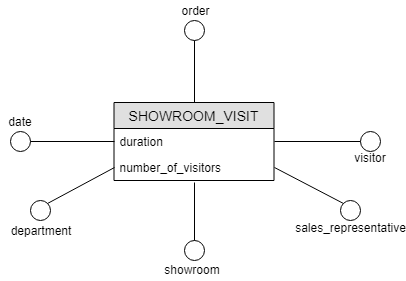
\includegraphics[scale=0.65]{../images/DFM_Showroom_Simple.png}
        \caption{
                \label{fig:showroom}  
                DFM of the showroom visit
        }
\end{figure}

\begin{figure}[H] 
        \centering
        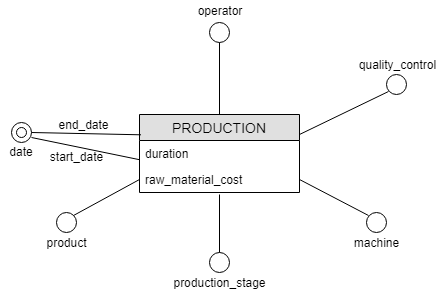
\includegraphics[scale=0.65]{../images/DFM_Production_Simple.png}
        \caption{
                \label{fig:production}  
                DFM of the production
        }
\end{figure}

\subsection{Showroom visit}

\begingroup
\renewcommand\arraystretch{0.5}
\begin{longtable}{p{3.7cm}p{10cm}}
        \caption{Fact table} \\
        Dimension & Attributes \\
        \endfirsthead \\
        Dimension & Attributes \\
        \endhead \\
        \hline \\
        Date & Day, Month, Year, Quartal, Week, Day of Week, Season, Holiday \\
        \hline \\
        Showroom & Name, City, District, Province, Region, Country, Manager, Address, Telephone, Size \\
        \hline \\
        Visitor & Name, City, District, Province, Region, Country, Language, Telephone, E-Mail, Type, Sector, Gender, Customer number \\
        \hline \\
        Order & Order Number, Total Price, Discount \\
        \hline \\
        Order Detail & Quantity, Quantity Type, Product, Unit price, Total price \\
        \hline \\
        Department & Name \\
        \hline \\
        Sales representative & Name, City, District, Province, Region, Country, Language, Telephone, E-Mail, Gender \\
        \hline \\
\end{longtable}
\endgroup

\begin{figure}[H] 
        \centering
        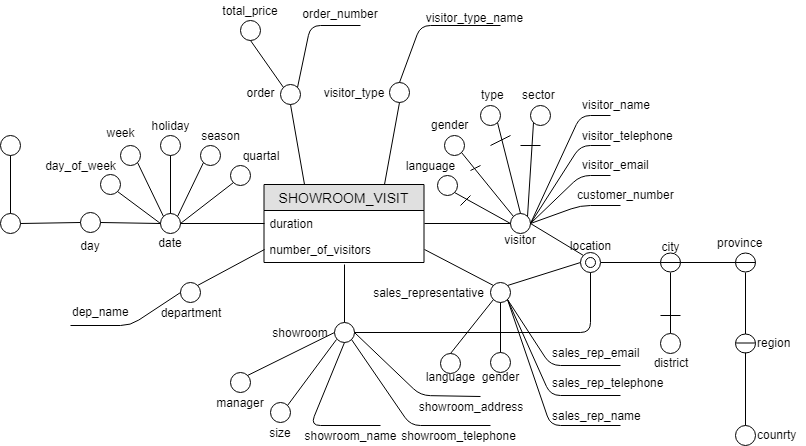
\includegraphics[width=\columnwidth]{../images/DFM_Showroom.png}
        \caption{
                \label{fig:showroomAttributes}  
                Dimension fact model (DFM) of the showroom visit with attributes 
        }
\end{figure}

\subsection{Production}

\begingroup
\renewcommand\arraystretch{0.5}
\begin{longtable}{p{4cm}p{9cm}}
        \caption{Fact table} \\
        Dimension & Attributes \\
        \endfirsthead \\
        Dimension & Attributes \\
        \endhead \\
        \hline \\
        Start date & Day, Month, Year, Week \\
        \hline \\
        End date & Day, Month, Year, Week \\
        \hline \\
        Product & Product number, Name, Department, Category \\
        \hline \\
        Production stage & Name \\
        \hline \\
        Machine & Name, Purchasing year, Vendor \\
        \hline \\
        Quality control & Grade \\
        \hline \\
        Operator & Name \\
        \hline \\
\end{longtable}
\endgroup

\begin{figure}[h] 
        \centering
        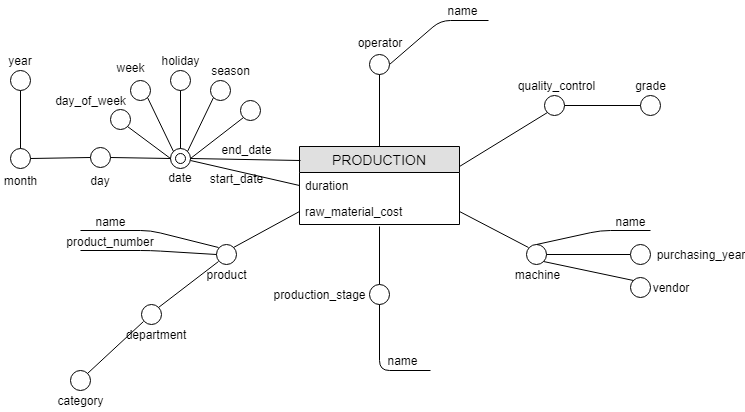
\includegraphics[width=\columnwidth]{../images/DFM_Production.png}
        \caption{
                \label{fig:productionAttributes}  
                Dimension fact model (DFM) of the production with attributes 
        }
\end{figure}

\section{Logical Design}

\subsection{Star schemas}

The following star schema fig. \ref{fig:starschemaShowroom} represent the first business process, namely the showroom visit.

\begin{figure}[h] 
        \centering
        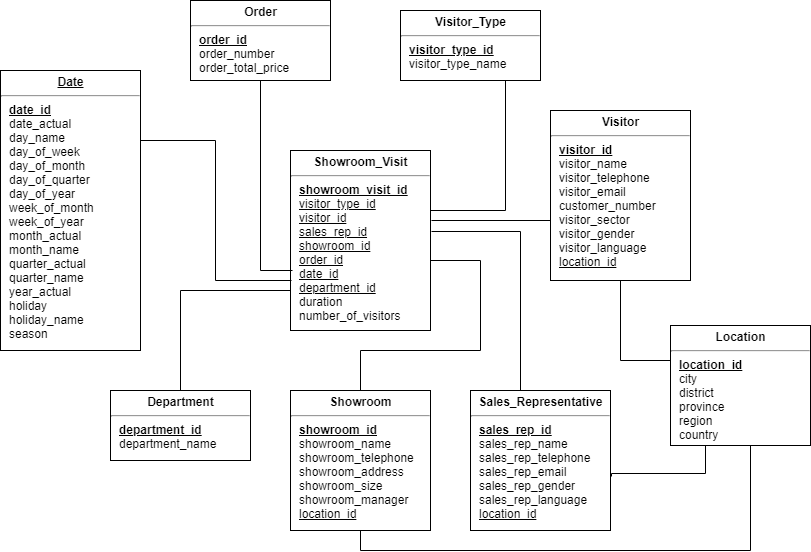
\includegraphics[width=\columnwidth]{../images/Starschema_Showroom_visit.png}
        \caption{
                \label{fig:starschemaShowroom}  
                Star schema of the showroom visit
        }
\end{figure}

Instead, the star schema fig. \ref{fig:starschemaProduction} represents the production business process.

\begin{figure}[h] 
        \centering
        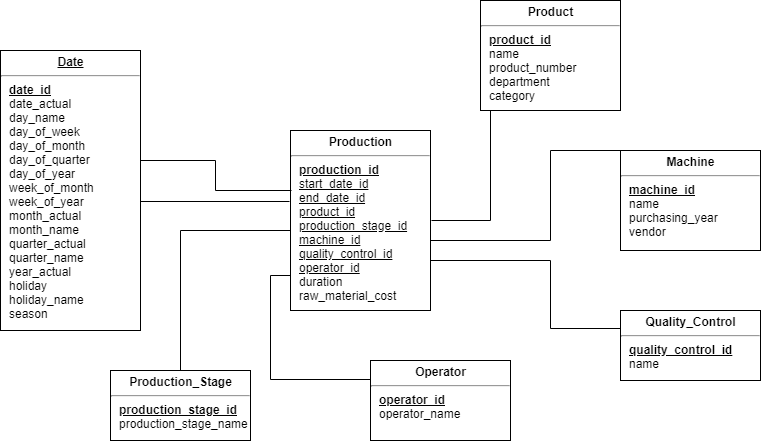
\includegraphics[width=\columnwidth]{../images/Starschema_Production.png}
        \caption{
                \label{fig:starschemaProduction}  
                Star schema of the production
        }
\end{figure}

\subsection{Two business questions}

\subsubsection{Fact: Showroom visit}

In order to be able to make the right marketing decisions, it is very important for the management to know from which sector the various customers or interested parties of a particular showroom come from. So, for example the management wants to know, from which sectors the various customers of showroom "Showroom-Bozen" were coming in the last year.

\bigskip
\noindent SQL query:
\begin{lstlisting}[
        language=SQL,
        showspaces=false,
        basicstyle=\ttfamily,
        numbers=left,
        numberstyle=\tiny,
        commentstyle=\color{gray}
     ]
SELECT v.visitor_sector, count(*)
FROM warehouse.visitor v
INNER JOIN warehouse.showroom_visit sv on v.visitor_id = sv.visitor_id
INNER JOIN warehouse.showroom s on sv.showroom_id = s.showroom_id
INNER JOIN warehouse.date d on sv.date_id = d.date_id
WHERE s.showroom_name = 'Showroom-BOZEN' 
AND d.date_actual >= '2018-01-01' AND d.date_actual <= '2018-12-31'
GROUP by v.visitor_sector
\end{lstlisting}

\begingroup
\renewcommand\arraystretch{0.5}
\begin{longtable}{p{1.4cm}p{1.5cm}p{1.8cm}p{1.5cm}p{1.6cm}p{1.4cm}p{1.2cm}p{1.25cm}p{1.85cm}}
        \caption{Showroom visit} \\
        ID & Visitor\_id & Sales\_rep\_id & Showr.\_id & Depart.\_id & Date\_id & Type\_id & Duration & Nr.\_of\_visit. \\
        \endfirsthead \\
        ID & Visitor\_id & Sales\_rep\_id & Showr.\_id & Depart.\_id & Date\_id & Type\_id & Duration & Nr.\_of\_visit. \\
        \endhead \\
        \hline \\
        1282369	& \color{red} 570822 & 6 & \color{red} 5 & 4 & \color{red}20180323 & 2 & 90 & 2 \\
        \hline \\
        1282370	& 570823 & 5 & 5 & 2 & 20160107 & 4 & 167 & 4 \\
        \hline \\
        1282371	& 570823 & 7 & 5 & 1 & 20130526 & 3 & 173 & 6 \\
        \hline \\
        1282372	& 570823 & 11 & 5 & 6 & 20150806  & 3 & 100 & 10 \\
        \hline \\
        1282373	& 570823 & 7 & 5 & 1 & 20121116 & 4 & 169 & 5 \\
        \hline \\
        1282374	& 570824 & 7 & 5 & 1 & 20171210 & 3 & 57 & 3 \\
        \hline \\
        1282375	& 570824 & 18 & 5 & 2 & 20110212 & 3 & 166 & 7 \\
        \hline \\
        1282376	& 570824 & 9 & 5 & 4 & 20130811  & 3 & 84 & 5 \\
        \hline \\
        1282377	& 570825 & 11 & 5 & 6 & 20170507 & 3 & 184 & 10 \\
        \hline \\
        1282378	& 570825 & 12 & 5 & 2 & 20111127 & 2 & 26 & 2 \\
        \hline \\
        1282379	& 570825 & 7 & 5 & 1 & 20150425 & 3 & 141 & 10 \\
        \hline \\
        1282380	& 570826 & 11 & 5 & 6 & 20130208 & 2 & 8 & 2 \\
        \hline \\
        1282381	& 570826 & 12 & 5 & 1 & 20111214 & 3 & 61 & 8 \\
        \hline \\
        1282382	& 570827 & 12 & 5 & 1 & 20170202 & 3 & 139 & 9 \\
        \hline \\
        1282383 & 570827 & 12 & 5 & 2 & 20121012 & 3 & 71 & 7 \\
        \hline \\
\end{longtable}
\endgroup

\begingroup
\renewcommand\arraystretch{0.5}
\begin{longtable}{p{1.3cm}p{1.6cm}p{1.8cm}p{3.6cm}p{2cm}p{.7cm}p{1.2cm}p{1.4cm}}
        \caption{Visitor} \\
        ID & Name & Telephone & E-Mail & Sector & Sex & Lang. & Loc.\_id \\
        \endfirsthead \\
        ID & Name & Telephone & E-Mail & Sector & Sex & Lang. & Loc.\_id \\
        \endhead \\
        \hline \\
        \color{red} 570822 & Melanie Eder &  &  & \color{red} Gastronomy & F & german & 9 \\
        \hline \\
        570823 & Julian Schmidt &  & j.schmidt@email.com & \color{red} Private & M & german & 9 \\
        \hline \\
        570824 & Marcel Schwarz & 306 9579783 & m.schwarz@email.com & \color{red} Hotel & M & german & 9 \\
        \hline \\
        570825 & Denise Fuchs & 396 5305260 & d.fuchs@email.com & \color{red} Public & F & german & 9 \\
        \hline \\
        570826 & Sophie Wimmer & 322 7641804 & s.wimmer@email.com & \color{red} Private & F & german & 9 \\
        \hline \\
\end{longtable} 
\endgroup

\begingroup
\renewcommand\arraystretch{0.5}
\begin{longtable}{p{0.25cm}p{3.9cm}p{2.2cm}p{2.9cm}p{.7cm}p{3.1cm}p{1.1cm}}
        \caption{Showroom} \\
        ID & Name & Telephone & Address & Size & Manager & Loc.\_id \\
        \endfirsthead \\
        ID & Name & Telephone & Address & Size & Manager & Loc.\_id \\
        \endhead \\
        \hline \\
        1 & Showroom-LATSCH & 0477 069655 & Herrengasse 8 & 581 & Paul Wolf & 42 \\
        \hline \\
        2 & Showroom-M{\"U}HLBACH & 0474 039227 & Platzerstr. 58 & 349 & Christoph Steiner & 54 \\
        \hline \\
        3 & Showroom-M{\"O}LTEN & 0470 429676 & Vernag 97 & 857 & Christoph Steiner & 51 \\
        \hline \\
        4 & Showroom-SALURN & 0475 248487 & Gewerbezone 44 & 198 & Johannes Egger & 77 \\
        \hline \\
        \color{red} 5 & \color{red} Showroom-BOZEN & 0473 723301 & St. Urban 73 & 447 & Sabine Schneider & 9 \\
        \hline \\
\end{longtable} 
\endgroup

\begingroup
\renewcommand\arraystretch{0.5}
\begin{longtable}{p{1.5cm}p{2cm}p{1.5cm}p{1.5cm}p{1.3cm}p{1.1cm}p{0.7cm}p{1.1cm}p{1.2cm}}
        \caption{Date} \\
        ID & Date & Day\_week & Day & Month & Quartal & Year & Holiday & Season \\
        \endfirsthead \\
        ID & Date & Day\_week & Day & Month & Quartal & Year & Holiday & Season \\
        \endhead \\
        \hline \\
        20160102 & 2010-01-02 & 6 & Saturday & January & First & 2016 & false & Winter \\
        \hline \\
        20170103 & 2010-01-03 & 7 & Sunday & January & First & 2017 & false & Winter \\
        \hline \\
        20180108 & \color{red} 2018-01-08 & 5 & Friday & January & First & 2018 & false & Winter \\
        \hline \\
        20190109 & 2010-01-09 & 6 & Saturday & January & First & 2019 & false & Winter \\
        \hline \\
        20200110 & 2010-01-10 & 7 & Sunday & January & First & 2020 & false & Winter \\
        \hline \\
\end{longtable} 
\endgroup

\begingroup
\renewcommand\arraystretch{0.5}
\begin{longtable}{p{3cm}p{4cm}}
        \caption{Result of the query} \\
        Sector & Number of visitors \\
        \endfirsthead \\
        Sector & Number of visitors \\
        \endhead \\
        \hline \\
        Gastronomy & 2985 \\
        \hline \\
        Hotel & 4223 \\
        \hline \\
        Private & 5629 \\
        \hline \\
        Public & 1371 \\
        \hline \\
\end{longtable} 
\endgroup

\subsubsection{Fact: Production}

The company's quality control is always interested in optimizing processes. It is therefore interesting for employees to know whether a machine has significant time differences in production in relation to a particular product in comparison to the other machines.

\bigskip
\noindent SQL query:
\begin{lstlisting}[
        language=SQL,
        showspaces=false,
        basicstyle=\ttfamily,
        numbers=left,
        numberstyle=\tiny,
        commentstyle=\color{gray}
     ]
SELECT m.machine_name, avg(p.duration) AS avg_production_duration
FROM warehouse.machine m
INNER JOIN warehouse.production p ON m.machine_id = p.machine_id
INNER JOIN warehouse.product o ON p.product_id = o.product_id
WHERE o.product_number = 'Warteraum-Couch - 10'
GROUP BY m.machine_id
ORDER BY avg_production_duration DESC LIMIT 10
\end{lstlisting}

\begingroup
\renewcommand\arraystretch{0.5}
\begin{longtable}{p{1cm}p{1.5cm}p{1.5cm}p{1cm}p{1.5cm}p{1.8cm}p{1.6cm}p{1.3cm}p{2.2cm}}
        \caption{Production} \\
        ID & Operator* & Machine* & Stage* & Product* & Start\_date* & End\_date* & Duration & Raw\_mat.\_cost \\
        \endfirsthead \\
        ID & Operator* & Machine* & Stage* & Product* & Start\_date* & End\_date* & Duration & Raw\_mat.\_cost \\
        \endhead \\
        \hline \\
        591814 & 779 & 1144 & 1 & \color{red} 361016 & 20101105 & 20101202 & \color{red} 152 & 76 \\
        \hline \\
        591815 & 780 & 1174 & 2 & \color{red} 361016 & 20101202 & 20101203 & \color{red} 1 & 395 \\
        \hline \\
        591816 & 775 & 1213 & 3 & \color{red} 361016 & 20101203 & 20101207 & \color{red} 2 & 277 \\
        \hline \\
        591817 & 770 & 1055 & 1 & \color{red} 361016 & 20101122 & 20101214 & \color{red} 30 & 66 \\
        \hline \\
        591818 & 722 & \color{red} 1176 & 2 & \color{red} 361016 & 20101214 & 20110111 & \color{red} 133 & 391 \\
        \hline \\
        591819 & 755 & 1079 & 3 & \color{red} 361016 & 20110111 & 20110204 & \color{red} 36 & 275 \\
        \hline \\
        591820 & 740 & 1069 & 1 & \color{red} 361016 & 20150511 & 20150520 & \color{red} 49 & 73 \\
        \hline \\
        591821 & 756 & 1025 & 2 & \color{red} 361016 & 20150520 & 20150603 & \color{red} 54 & 398 \\
        \hline \\
        591822 & 758 & 1130 & 3 & \color{red} 361016 & 20150603 & 20150625 & \color{red} 96 & 278 \\
        \hline \\
        27064 & 754 & 1164 & 1 & \color{red} 361016 & 20101022 & 20101026 & \color{red} 8 & 66 \\
        \hline \\
        27065 & 739 & 1028 & 2 & \color{red} 361016 & 20101026 & 20101104 & \color{red} 6 & 407 \\
        \hline \\
        27066 & 798 & 1098 & 3 & \color{red} 361016 & 20101104 & 20101105 & \color{red} 6 & 280 \\
        \hline \\
        27067 & 780 & 1013 & 1 & \color{red} 361016 & 20130327 & 20130411 & \color{red} 70 & 74 \\
        \hline \\
        27068 & 737 & 1145 & 2 & \color{red} 361016 & 20130411 & 20130509 & \color{red} 18 & 404 \\
        \hline \\
        27069 & 772 & 1032 & 3 & \color{red} 361016 & 20130509 & 20130520 & \color{red} 14 & 281 \\
        \hline \\
\end{longtable} 
\endgroup

Note: all columns with the * are foreign key columns and are carrying only the id

\begingroup
\renewcommand\arraystretch{0.5}
\begin{longtable}{p{1cm}p{3cm}p{3.2cm}p{3.1cm}}
        \caption{Machine} \\
        ID & Machine\_name & Machine\_vendor & Purchasing\_year \\
        \endfirsthead \\
        ID & Machine\_name & Machine\_vendor & Purchasing\_year \\
        \endhead \\
        \hline \\
        1172 & Melichár & Durán & 1998 \\
        \hline \\
        1173 & Horn & Lóntos & 2009 \\
        \hline \\
        1174 & Chihaia & Murtazaev & 2002 \\
        \hline \\
        1175 & Korčák & Durán & 2006 \\
        \hline \\
        \color{red} 1176 & \color{red} Ramóna & Barbora & 1996 \\
        \hline \\
\end{longtable} 
\endgroup

\begingroup
\renewcommand\arraystretch{0.5}
\begin{longtable}{p{1.4cm}p{2.7cm}p{3.7cm}p{3.4cm}p{3cm}}
        \caption{Product} \\
        ID & Product\_name & Product\_number & Product\_department & Product\_category \\
        \endfirsthead \\
        ID & Product\_name & Product\_number & Product\_department & Product\_category \\
        \endhead \\
        \hline \\
        361013 & Warteraum-Couch & Warteraum-Couch - 7 & Büro & Arztpraxis-Set \\
        \hline \\
        361014 & Warteraum-Couch & Warteraum-Couch - 8 & Büro & Arztpraxis-Set \\
        \hline \\
        361015 & Warteraum-Couch & Warteraum-Couch - 9 & Büro & Arztpraxis-Set \\
        \hline \\
        \color{red} 361016 & Warteraum-Couch & \color{red} Warteraum-Couch - 10 & Büro & Arztpraxis-Set \\
        \hline \\
        361017 & Warteraum-Couch & Warteraum-Couch - 11 & Büro & Arztpraxis-Set \\
        \hline \\
\end{longtable} 
\endgroup

\begingroup
\renewcommand\arraystretch{0.5}
\begin{longtable}{p{3cm}p{4cm}}
        \caption{Result of the query} \\
        Machine\_name & AVG\_Production\_duration \\
        \endfirsthead \\
        Machine\_name & AVG\_Production\_duration \\
        \endhead \\
        \hline \\
        Vajda & 152.00 \\
        \hline \\
        \color{red} Ramóna & 133.00 \\
        \hline \\
        Papandreou & 96.00 \\
        \hline \\
        Kontoléon & 70.00 \\
        \hline \\
        Mitu & 54.00 \\
        \hline \\
        Bercu & 49.00 \\
        \hline \\
        Heinrich & 36.00 \\
        \hline \\
        Martinez & 30.00 \\
        \hline \\
        Pál & 18.00 \\
        \hline \\
        Aguilar & 14.00 \\
        \hline \\
\end{longtable} 
\endgroup

\section{Implementation}
\subsection{ROLLUP}
\subsubsection{SQL query using ROLLUP for business process 1 (showroom visit)}

The following sql query shows the number of visitors per showroom, in the different areas and in the different seasons. In addition there are the different partial sums. For example, for the showroom in Bolzano, first the number of visitors for the 'bBedroom' area in autumn is shown, then the total number of visitors for the 'bedroom' area, regardless of the season, and finally the total number of visitors for the showroom in Bolzano, regardless of the area and the season.

\begin{lstlisting}[
        language=SQL,
        showspaces=false,
        basicstyle=\ttfamily,
        numbers=left,
        numberstyle=\tiny,
        commentstyle=\color{gray}
     ]
SELECT showroom_name, department_name, season, count(visitor_id)
FROM warehouse.showroom_visit
JOIN warehouse.showroom using (showroom_id)
JOIN warehouse.department using (department_id)
JOIN warehouse.date using (date_id)
GROUP BY ROLLUP(showroom_name, department_name, season);
\end{lstlisting}

\subsubsection{SQL query with ROLLUP for business process 2 (production)}

The following sql query shows the average machining time for a particular production stage of a particular product of a particular product category. The query also returns the average machining times of the higher levels, in other words, a granularity is removed step by step. For example, the average machining time of 'table XY' is shown first for the 'fine grinding' process. Then you get the average machining time of all processes on 'table XY' and finally the average machining time of all processes on all table models, thus of the whole product category 'table'.

\begin{lstlisting}[
        language=SQL,
        showspaces=false,
        basicstyle=\ttfamily,
        numbers=left,
        numberstyle=\tiny,
        commentstyle=\color{gray}
     ]
SELECT product_category, product_name, 
        production_stage_name, ROUND(avg(duration)::numeric,2)
FROM warehouse.production
JOIN warehouse.product using (product_id)
JOIN warehouse.production_stage using (production_stage_id)
GROUP BY ROLLUP(product_category, product_name, production_stage_name);
\end{lstlisting}    

\subsection{CUBE}

\subsubsection{SQL query using CUBE for business process 1 (showroom visit)}

The following query shows the number of visitors from the province of Bolzano and its commercial sector in the different districts of the showrooms. In addition, the query shows all possible sub-totals, removing step by step different granularities. In other words, for each combination of values, the sum is shown, finally the total sum of all visits from visitors from the province of Bolzano.

\begin{lstlisting}[
        language=SQL,
        showspaces=false,
        basicstyle=\ttfamily,
        numbers=left,
        numberstyle=\tiny,
        commentstyle=\color{gray}
        ]
SELECT visitor_sector, vl.district, sl.district, 
        sum(number_of_visitors)
FROM warehouse.showroom_visit
JOIN warehouse.visitor using (visitor_id)
JOIN warehouse.location as vl 
        on warehouse.visitor.location_id = vl.location_id 
JOIN warehouse.showroom using (showroom_id)
JOIN warehouse.location as sl 
        on warehouse.showroom.location_id = sl.location_id
WHERE vl.province = 'Bozen'
GROUP BY CUBE(vl.district, visitor_sector, sl.district)
ORDER BY visitor_sector, vl.district, sl.district;
\end{lstlisting}    

\subsubsection{SQL query using CUBE for business process 2 (production)}

The following query shows the average grade of the quality control for a machine and for the product category. Also all partial average values of all different combinations and groupings can be read off.

\begin{lstlisting}[
        language=SQL,
        showspaces=false,
        basicstyle=\ttfamily,
        numbers=left,
        numberstyle=\tiny,
        commentstyle=\color{gray}
     ]
SELECT product_department, machine_name, 
        ROUND(avg(quality_control_grade)::numeric,2)
FROM warehouse.production
JOIN warehouse.product using (product_id)
JOIN warehouse.machine using (machine_id)
JOIN warehouse.quality_control using (quality_control_id)
WHERE quality_control_grade is not NULL
GROUP BY CUBE(product_department, machine_name)
ORDER BY avg(quality_control_grade) desc;	
\end{lstlisting}

\subsection{GROUPING SETS}

\subsubsection{SQL query using GROUPING SETS for business process 1 (showroom visit)}

The following query shows the number of visitors per language served by a sales representative in a showroom. Also the total number of visitors can be taken from a language in that showroom as well as the total number of visitors served by that sales representative.

\begin{lstlisting}[
        language=SQL,
        showspaces=false,
        basicstyle=\ttfamily,
        numbers=left,
        numberstyle=\tiny,
        commentstyle=\color{gray}
        ]
SELECT showroom_name, sales_rep_name, 
        visitor_language, sum(order_total_price)
FROM warehouse.showroom_visit
JOIN warehouse.visitor using (visitor_id)
JOIN warehouse.sales_representative using (sales_rep_id)
JOIN warehouse.order using (order_id)
JOIN warehouse.showroom using (showroom_id)
GROUP BY GROUPING SETS(
        (showroom_name, sales_rep_name, visitor_language),
        (showroom_name, visitor_language),
        (showroom_name, sales_rep_name));
\end{lstlisting}          

\subsubsection{SQL query using GROUPING SETS for business process 2 (production)}

The following query shows the number of a certain grade for a product category in a specific year. The query also shows the number of a certain rating in a certain year.

\begin{lstlisting}[
        language=SQL,
        showspaces=false,
        basicstyle=\ttfamily,
        numbers=left,
        numberstyle=\tiny,
        commentstyle=\color{gray}
        ]
SELECT product_category, year_actual, 
        quality_control_grade, count(product_id)
FROM warehouse.production
JOIN warehouse.product using (product_id)
JOIN warehouse.date ON date.date_id = production.end_date_id
JOIN warehouse.quality_control using (quality_control_id)
GROUP BY GROUPING SETS(
        (product_category, year_actual, quality_control_grade),
        (year_actual, quality_control_grade));
\end{lstlisting}

\section{Querying}

\subsection{NTILE}

\subsubsection{SQL query using NTILE for business process 1 (showroom visit)}

The following sql statement calculates the number of visitors coming from a particular location of the province of Bolzano and assigns each row to a group from 1-4, depending on the size of the number of visitors.

\begin{lstlisting}[
        language=SQL,
        showspaces=false,
        basicstyle=\ttfamily,
        numbers=left,
        numberstyle=\tiny,
        commentstyle=\color{gray}
        ]	 
SELECT vl.city, count(visitor_id), 
        NTILE(4) OVER (ORDER BY count(visitor_id)) AS TILE4
FROM warehouse.showroom_visit
JOIN warehouse.visitor using (visitor_id)
JOIN warehouse.location as vl 
        on warehouse.visitor.location_id = vl.location_id 
WHERE vl.province = 'Bozen'
GROUP BY vl.city;
\end{lstlisting}
      
\subsubsection{SQL query using NTILE for business process 2 (production)}

The next sql query sums all processing times of an operator and groups them to 4 groups, were each operators gets assigned to a specific group relatively to the sum of duration of all production steps.

\begin{lstlisting}[
        language=SQL,
        showspaces=false,
        basicstyle=\ttfamily,
        numbers=left,
        numberstyle=\tiny,
        commentstyle=\color{gray}
        ]
SELECT operator_name, ROUND(sum(duration)::numeric,2), 
        NTILE(4) OVER (ORDER BY sum(duration)) AS TILE4
FROM warehouse.production
JOIN warehouse.operator using (operator_id)
GROUP BY operator_name;
\end{lstlisting}

\subsection{RANK}

\subsubsection{SQL query using RANK for business process 1 (showroom visit)}

The following query identifies the overall total number of visitors per showroom and ranks them according to their number of visitors.

\begin{lstlisting}[
        language=SQL,
        showspaces=false,
        basicstyle=\ttfamily,
        numbers=left,
        numberstyle=\tiny,
        commentstyle=\color{gray}
        ]
SELECT showroom_name, count(distinct visitor_id), 
        RANK() OVER (ORDER BY count(distinct visitor_id) DESC)
FROM warehouse.showroom_visit
JOIN warehouse.showroom using (showroom_id)
GROUP BY showroom_name;
\end{lstlisting}

\subsubsection{SQL query using RANK for business process 2 (production)}

The following sql query ranks the different products with respect to their average raw material costs.

\begin{lstlisting}[
        language=SQL,
        showspaces=false,
        basicstyle=\ttfamily,
        numbers=left,
        numberstyle=\tiny,
        commentstyle=\color{gray}
        ]
SELECT product_category, ROUND(avg(raw_material_cost)::numeric,2),
        RANK() OVER (ORDER BY (avg(raw_material_cost)) DESC)
FROM warehouse.production
JOIN warehouse.product using (product_id)
GROUP BY product_category;
\end{lstlisting}
                
\subsection{??????}

\subsubsection{SQL query ??????}

(text missing)

\begin{lstlisting}[
        language=SQL,
        showspaces=false,
        basicstyle=\ttfamily,
        numbers=left,
        numberstyle=\tiny,
        commentstyle=\color{gray}
        ]																			   
SELECT date_actual, sum(order_total_price), 
        ROUND(AVG(SUM(order_total_price))
                OVER ( ORDER BY date_actual
                ROWS BETWEEN 7 PRECEDING
                AND CURRENT ROW)::numeric,2)
FROM warehouse.showroom_visit
JOIN warehouse.date using (date_id)
JOIN warehouse.order using (order_id)
WHERE year_actual > 2017
GROUP BY date_actual
ORDER BY date_actual;
\end{lstlisting}				  
                
\subsubsection{SQL query ??????}

(text missing)

\begin{lstlisting}[
        language=SQL,
        showspaces=false,
        basicstyle=\ttfamily,
        numbers=left,
        numberstyle=\tiny,
        commentstyle=\color{gray}
        ]			  
SELECT year_actual, month_actual, sum(raw_material_cost), 
        ROUND(AVG(SUM(raw_material_cost))
                OVER ( ORDER BY year_actual, month_actual
                ROWS BETWEEN 6 PRECEDING
                AND CURRENT ROW)::numeric,2)
FROM warehouse.production
JOIN warehouse.date ON date.date_id = production.end_date_id
GROUP BY year_actual, month_actual
ORDER BY year_actual, month_actual;	
\end{lstlisting}				  
        
\subsection{??????}

\subsubsection{SQL query ??????}

(text missing)

\begin{lstlisting}[
        language=SQL,
        showspaces=false,
        basicstyle=\ttfamily,
        numbers=left,
        numberstyle=\tiny,
        commentstyle=\color{gray}
        ]
SELECT year_actual, quarter_actual, 
visitors_this_year, visitors_last_year,
visitors_this_year - visitors_last_year as difference
FROM (
        SELECT year_actual, quarter_actual,
                count(visitor_id) as visitors_this_year,
                LAG(count(visitor_id), 4) 
                OVER (ORDER BY year_actual, quarter_actual) 
                as visitors_last_year 
        FROM warehouse.showroom_visit
                JOIN warehouse.date using (date_id)
                JOIN warehouse.order using (order_id)
                GROUP BY year_actual, quarter_actual
                ORDER BY year_actual, quarter_actual) as last_year
        WHERE year_actual > 2010;
\end{lstlisting}

\section{Data Analysis Tool}


% \bibliography{references}{}
% \bibliographystyle{plain}

\end{document}